% Chapter Template

\chapter{Simulation Physics} % Main chapter title

\label{ch:models} % Change X to a consecutive number; for referencing this chapter elsewhere, use \ref{ChapterX}

\lhead{Chapter 2. \emph{Simulation Physics}} % Change X to a consecutive number; this is for the header on each page - perhaps a shortened title

%----------------------------------------------------------------------------------------
%	SECTION 1
%----------------------------------------------------------------------------------------

\section{Simulations Used}
To demonstrate the efficacy of the various uncertainty quantification methods we use in this work, we employ
several independent simulations (hereafter referred to as ``codes'') of increasing complexity.  These codes
range from simple polynomial evaluations to analytic solutions of simple physics, to nonlinear multistage
iterative solvers representing complex codes.  We describe each briefly here.


\section{Polynomial Evaluations}
In order to benchmark the simplest cases, we make use of simple polynomial expressions of the form
\begin{equation}
  u(Y) = \prod_{n=1}^N (y_n+1),
\end{equation}
where $u(Y)$ is the quantity of interest and $Y=[y_1,y_2,\ldots,y_N]$ is the vector of uncertain inputs.
The input variables $Y$ can be distributed arbitrarily; we distribute them uniformly from -1 to 1.  This
results in an isotropic hypercube domain extending from -1 to 1 in all dimensions.  
Because this model is a sum of polynomials, SCgPC can represent it exactly.  Because it is highly regular, we
also expect SCgPC to be efficient.





\section{Attenuation}
To demonstrate the convergence rates of various methods, we make use of an attenuation problem that
is equivalent to the penetration of neutral particles in a one-dimensional purely-absorbing medium.  For this
problem we set the physical domain to $x\in[0,1]$, with the material occupying all of the domain space.  If $m$
particles are incident on a material with length $dx$, the resulting change in the number of particles $dm$
due to absorption is
\begin{equation}
  dm = -y m dx,
\end{equation}
where $y$ is the absorption cross section (probability of absorption per unit length) of the neutral particles
in the material.  The solution for the fraction of particles still present after passing through the material
for any position $x$ is
\begin{equation}
  m(x) = e^{-yx}.
\end{equation}
To expand the number of input parameters to the problem, we subdivide the material into $N$ independent
materials indexed by $n$, each with absorption cross section $y_n$ and length $h=\frac{1}{N}$.  We introduce uncertainty
by allowing each absorption cross section to vary uniformly between 0 and 1, resulting in a hypercubic
uncertainty domain.  We establish our quantity of interest as the percent of incident particles at the left
domain ($m(0)$) that remain after passing completely through the material ($m(L)$).  Introducing the
uncertain material properties as parameters for the quantity of interest, we define
\begin{equation}
  u(Y) = m(L,Y),\hspace{15pt}Y\equiv[y_1,\ldots,y_N].
\end{equation}
This subdivided domain model can be considered as distinct attenuation problems, where the fraction of
particles passing through one material are the full number incident on the next material.  Thus, the solution
is a product of the solutions to the one-dimension ODE,
\begin{align}
  u(Y) &= m_1(h,y_2)\cdot m_2(h,y_2)\cdot\ldots\cdot m_N(h,y_N),\\
    &= \prod_{n=1}^N e^{-h y_n},\\
    &= \prod_{n=1}^N e^{-y_n/N}.
\end{align}

The benefit of this model is a simple analytic solution, which makes analytic benchmarks straightforward to
compute.  In
addition, because of the exponential form, SCgPC will converge on a solution, but not replicate it exactly as
in the polynomial case.  This allows accurate comparison between MC, SCgPC methods, and HDMR methods in a
highly regular analytic case.

\section{Projectile}
For a nonlinear case without an analytic solution, we consider the path traveled by a projectile near the
surface of the Earth, considering drag on the projectile from stagnant air.  
The physical domain for this problem extends from $x=0,y=0$ as far as necessary for the projectile to reach
its apex and return to $y=0$.
The equations governing travel in both vertical position $x$ and horizontal position $y$
are given by
\begin{equation}
  y(t) = \frac{v_T}{g}(v\sin\theta+v_T)\left(1-\exp\left[\frac{-gt}{v_T}\right]\right)-v_T t,
\end{equation}
\begin{equation}
  x(t) = \frac{vv_T\cos\theta}{g}\left(1-\exp\left[\frac{-gt}{v_T}\right]\right),
\end{equation}
where $t$ is time, $g$ is acceleration due to gravity, $v$ is scalar velocity, $\theta$ the angle between the
velocity vector and the horizontal ground (x-axis), $v_T=\frac{mg}{D}$ is terminal velocity, $D=\frac{\rho CA}{2}$ is
the acceleration due to drag, $C$ is the drag coefficient, and $A=\pi r^2$
is the surface area of the projectile in the direction of travel.  The projectile is assumed to present an
identical surface area in both $x$ and $y$ directions.  The quantity of interest is the range, or the total
distance in $x$ traveled by the ball before reaching a height of $y=0$.  The uncertain input variables are
distributed uniformly as described in Table \ref{tab:proj dist}.

\begin{table}[h]
\centering
\begin{tabular}{c | l | c c | c}
  Variable & Name & Mean & Range ($\pm$) & Units \\\hline
  $y_i$ & Initial Height & 1 & 1 & m\\
  $v$ & Initial Velocity & 35.5 & 2.5 & m/s\\
  $\theta$ & Initial Angle & 45 & 10 & degrees\\
  $g$ & Accel. Gravity & 9.79888 & 0.0349 & m/s/s\\
  $m$ & Projectile Mass & 0.145 & 0.0725 & kg\\
  $r$ & Projectile Radius & 0.0336 & 0.00336 & m\\
  $C$ & Drag Coefficient & 0.5 & 0.5 & \\
  $\rho$ & Air Density & 1.2 & 0.1 & kg/m$^3$ \\
\end{tabular}
\caption{Projectile Problem Distributions}
\label{tab:proj dist}
\end{table}

This simulation has the benefit of an analytic solution when $C=0$ and eight distinct input parameters of
varying importance.  This is especially useful in considering anisotropic treatment of the input space.  The
regularity of the response is not well known, as there is no analytic solution to this case; however, we
expect the range to be less regular than the quantity of interest in the previous two cases.





\section{Neutron Diffusion}
For a nonlinear system with complicated physics, we consider a two-group, two-dimensional neutron diffusion
criticality calculation.  The physical domain for this problem extends along $x\in[0,165\text{ cm}]$ and
$y\in[0,165\text{ cm}]$.
We make use of the diffusion approximation for neutron transport, which when restricted to two energy groups provides us
with a coupled set of elliptic PDEs to solve:
\begin{equation}
-\grad\cdot\qty( D_1(\bar x)\grad\phi_1(\bar x))+\qty(\xs{a}{1}(\bar x)+\xs{s}{1\to2}(\bar x))\phi_1(\bar x) = \frac{1}{k(\phi)}\sum_{g'=1}^2\nu_{g'}\xs{f}{g'}(\bar x)\phi_{g'}(\bar x),
\end{equation}
\begin{equation}
-\grad \cdot\qty(D_2(\bar x)\grad \phi_2(\bar x))+\xs{a}{2}(\bar x)\phi_2(\bar x) = \xs{s}{1\to 2}(\bar x)\phi_1(\bar x),
\end{equation}
where we use the following parametric coefficients: 
the absorption cross section $\Sigma_{g,a}=\Sigma_{g,c}+\Sigma_{g,f}$; 
the capture and fission cross sections $\Sigma_{g,c}$ and $\Sigma_{g,f}$; 
the energy-group scattering cross section $\Sigma_s^{(g'\to g)}$; 
the diffusion coefficient $D_g$ which depends on the scattering cross section of the medium;
and the fission multiplication factor $\nu_g$, the ratio of new neutrons per fission-producing neutron.  The
solution to this PDE is the neutron scalar flux $\phi_g(\bar x)$.  We apply no-traction conditions on the
vacuum boundaries and zero-derivative current on the reflecting boundaries for both energy groups:
\begin{equation}
\frac{\phi_g}{4}-\frac{D_g}{2}\eval{\pdv{\phi_g}{x_1}}_{\partial \Omega_\text{top}}=0,\hspace{5pt} g=1,2,
\end{equation}
\begin{equation}
\frac{\phi_g}{4}-\frac{D_g}{2}\eval{\pdv{\phi_g}{x_2}}_{\partial \Omega_\text{right}}=0,\hspace{5pt} g=1,2,
\end{equation}
\begin{equation}
-D_g\eval{\pdv{\phi_g}{x_1}}_{\partial \Omega_\text{bottom}}=0,\hspace{5pt} g=1,2,
\end{equation}
\begin{equation}
-D_g\eval{\pdv{\phi_g}{x_2}}_{\partial \Omega_\text{left}}=0,\hspace{5pt} g=1,2.
\end{equation}
\\
The criticality eigenvalue and quantity of interest $k(\phi)$ is given by
\begin{equation}
k(\phi)=\sum_{g=1}^2\iint\limits_D\frac{\nu\xs{f}{g}\phi_g(\bar x)}{\qty(-\nabla\cdot D_g\nabla+\Sigma_r^{(g)})\phi_g(\bar x)}~d\bar x.
\end{equation}
We address solving $\phi_1,\phi_2,$ and $k$ nonlinearly and simultaneously using FEM and Jacobian-free
Newton-Krylov iterations.  
The material properties are shown in Table \ref{tab:coremats}, and the domain $\Omega=[0,200\text{ cm}]^2$.
The reference flux solutions are plotted in Fig. \ref{benchflux}, and for the reference problem
$k$=1.00007605445.  \begin{figure}[H]
\centering
  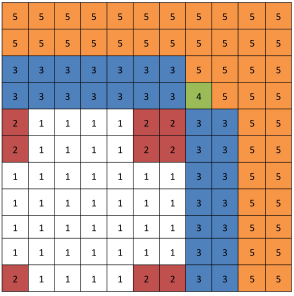
\includegraphics[width=0.4\linewidth]{core}
  \caption{Core Geometry}
  \label{geom}
\end{figure}
\begin{table}[h]
\centering
\begin{tabular}{c c | c c c c}
Region & Group & $D_g$ & $\Sigma_{a,g}$ & $\nu\Sigma_{f,g}$ & $\Sigma_s^{1,2}$ \\ \hline
1 & 1 & 1.255 & 8.252e-3 & 4.602e-3 & 2.533e-2 \\
 & 2 & 2.11e-1 & 1.003e-1 & 1.091e-1 & \\ \hline
2 & 1 & 1.268 & 7.181e-3 & 4.609e-3 & 2.767e-2 \\
 & 2 & 1.902e-1 & 7.047e-2 & 8.675e-2 & \\ \hline
3 & 1 & 1.259 & 8.002e-3 & 4.663e-3 & 2.617e-2 \\
 & 2 & 2.091e-1 & 8.344e-2 & 1.021e-1 & \\ \hline
4 & 1 & 1.259 & 8.002e-3 & 4.663e-3 & 2.617e-2 \\
 & 2 & 2.091e-1 & 7.3324e-2 & 1.021e-1 & \\ \hline
5 & 1 & 1.257 & 6.034e-4 & 0 & 4.754e-2 \\
 & 2 & 1.592e-1 & 1.911e-2 & 0 & 
\end{tabular}
\caption{Reference Material Properties for Benchmark Core}
\label{tab:coremats}
\end{table}
\begin{figure}[H]
\centering
  \begin{subfigure}[b]{0.45 \textwidth}
   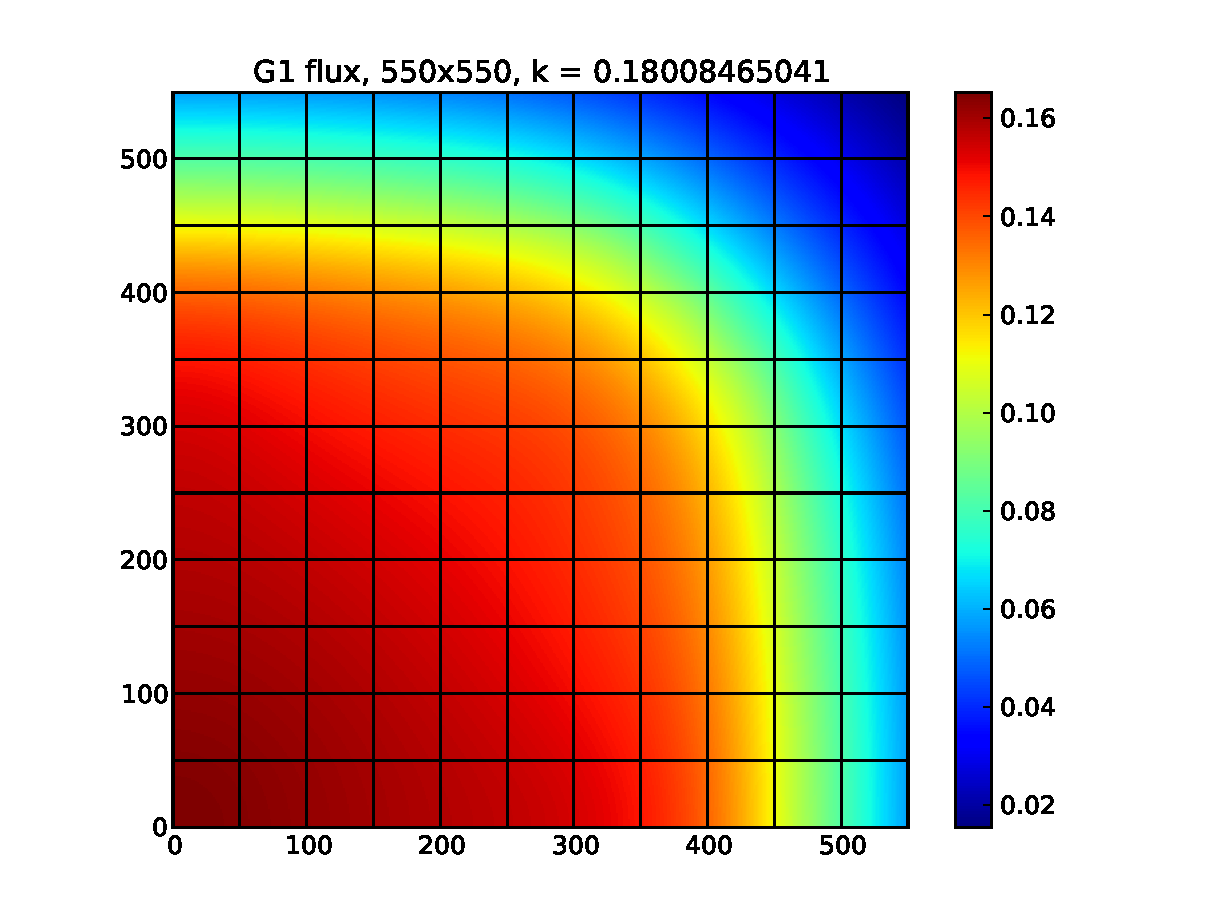
\includegraphics[width=\textwidth]{g1_50_flux}
   \caption{$\phi$, Group 1}
   \label{g1}
  \end{subfigure}
  \begin{subfigure}[b]{0.45 \textwidth}
   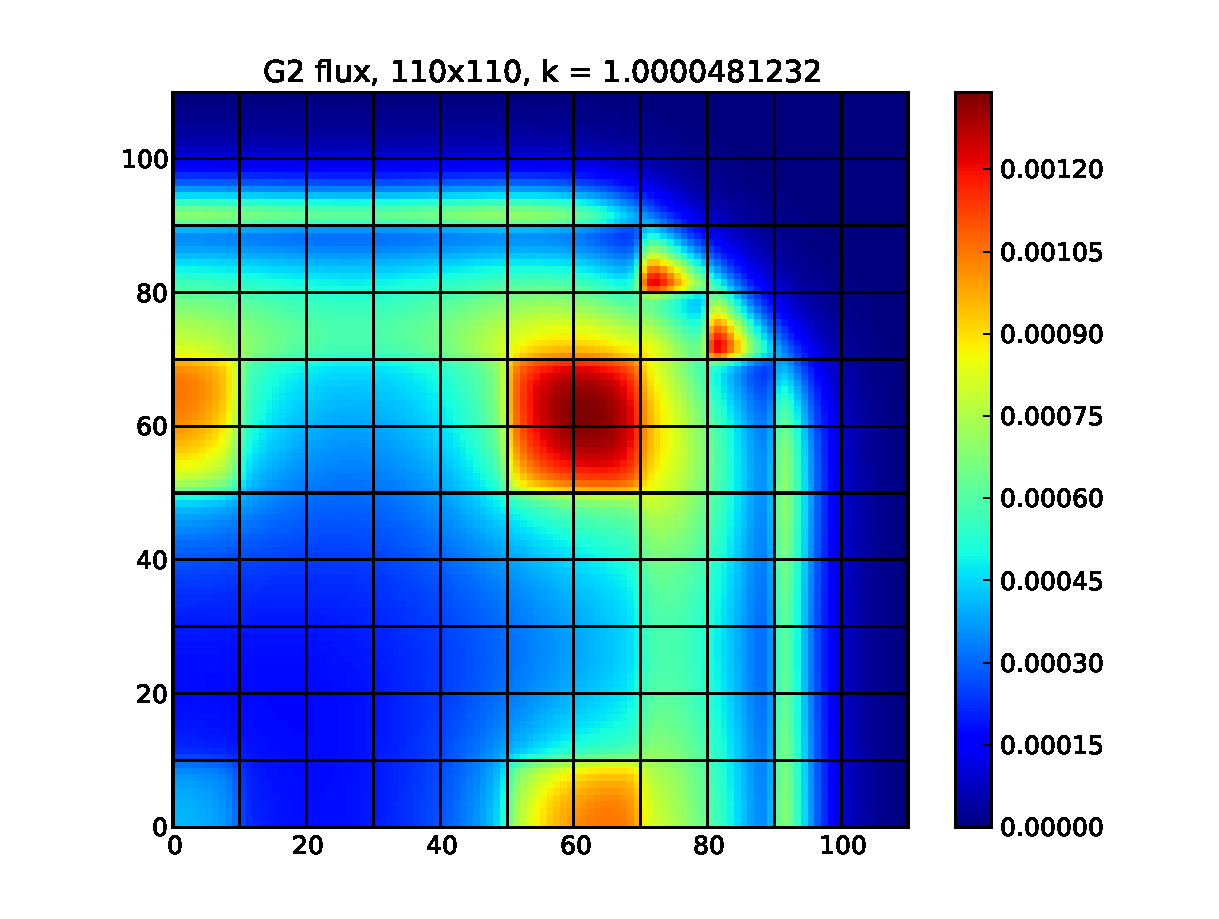
\includegraphics[width=\textwidth]{g2_50_flux}
   \caption{$\phi$, Group 2}
   \label{g2}
  \end{subfigure}
  \caption{Reference Flux Profiles}
  \label{benchflux}
\end{figure}
